%  Typ dokumentu - článek, prezentace aj.
\documentclass[english]{article}

%  Nastaví vstupní a výstupní kódování znaků (encoding) a lokalizace
\usepackage[T1]{fontenc}
\usepackage[utf8]{inputenc}
\usepackage[english,czech]{babel}
\usepackage{icomma}

%  Formát papíru a odsazení od jeho okrajů
\usepackage[letterpaper]{geometry}
\geometry{verbose,tmargin=1.5cm,bmargin=2cm,lmargin=2cm,rmargin=2cm}

%  Umožňuje pracovat s grafikou
\usepackage{graphicx}
\usepackage{bigstrut}
\usepackage{epstopdf}

%  Automaticky odsadí i první paragraf v každé sekci
\usepackage{indentfirst}

%  Umožňuje rozdělovat obsah na více sloupců
\usepackage{multicol}
\usepackage{booktabs}
\usepackage{pgffor}

%  Umožňuje používat hypertextové odkazy, nastavuje jejich barvu a vlastnosti
\usepackage[unicode]{hyperref}
\hypersetup{
	colorlinks=true, citecolor=blue, filecolor=blue, linkcolor=blue,
	urlcolor=blue
}

%  Umožnění odstranění italiky u jednotek
\newcommand{\unit}[1]{~\mathrm{#1}}
\newcommand{\unitb}[1]{~\mathrm{[#1]}}
\newcommand{\unitbr}[1]{\qquad\mathrm{[#1]}}

%  Formátování stránek, empty = odstraní číslování
% \pagestyle{empty}

%  Řádkování
\linespread{1.2}

%  Lepší zobrazování matematiky (rozšíření sum o \limits atd.)
%  Umožní psát přes \mathbb{N/R/Q/..} množiny čísel
\everymath{\displaystyle}
\usepackage{amsmath, amsthm, amssymb, wasysym}

%  Velikost fontu matematických výrazů v dokumentu lze pro danou
% základního fontu dokumentu upravit pomocí:
% \DeclareMathSizes{X}{Y}{Z}{U} kde:
% X je velikost fontu v dokumentu, pro kterou se matematika upraví
% Y je standartní velikost fontu matematiky
% Z je velikost fontu zmenšených (vnořených výrazů)
% U je velikost fontu ještě více zmenšených (vnořených výrazů).
\DeclareMathSizes{10}{10.5}{9}{9}

%  Nastaví autora, název, datum, skupinu měření apod. 
%  (můj vlastní příkaz, umožní znovu-použití v dokumentu)
\newcommand{\Author}{David Roesel}
\newcommand{\Coauthor}{Schönfeldová, Vyšín}
\newcommand{\Institute}{FJFI ČVUT v Praze}
\newcommand{\Subject}{VAKUOVÁ FYZIKA A TECHNIKA}
\newcommand{\Group}{Pá 14:30}
\newcommand{\Kruh}{FE}
\newcommand{\Title}{Úloha \#4  \\Čerpání vzduchu kryosorpční vývěvou}
\newcommand{\Date}{28.11.2014}

% Custom comands
\newcommand{\dd}{\mathrm{d}}
\newcommand{\dln}{\mathrm{ln}}
\newcommand{\ee}{\mathrm{e}}
\newcommand{\jelina}{Oooo, Jelina!}

% Začátek dokumentu - Formátování na výstup
\begin{document}

% Interní proměnné, možno zobrazovat u prezentací, používají se při
% generování pomocí \titlepage apod.
\author{\Author}
\title{\Title}
\date{\Date}

%  Lokalizace některých názvů do češtiny
\renewcommand{\figurename}{Obr.}
\renewcommand{\tablename}{Tab.}
\renewcommand{\refname}{Reference}

% --- Hlavička dokumentu -----------------------------------------------

\setlength{\parindent}{0cm}
\begin{multicols}{2}
\textbf{\Subject \\
        \Institute \\[0.1cm]
%\large  \Title \\[0.5cm]
\Title \\[0.5cm]
}
\begin{tabular}{rlrl}
\large Datum měření: & \Date & \large Skupina: & \Group \\
\large Jméno: & \Author & \large Kroužek:  & \Kruh\\
\large Spolupracovali: & \Coauthor &\large Klasifikace:\\
\end{tabular}

\begin{flushright}

\includegraphics[scale=0.28]{../../_meta/fjfi_standart.pdf}
\hspace{0.2cm}
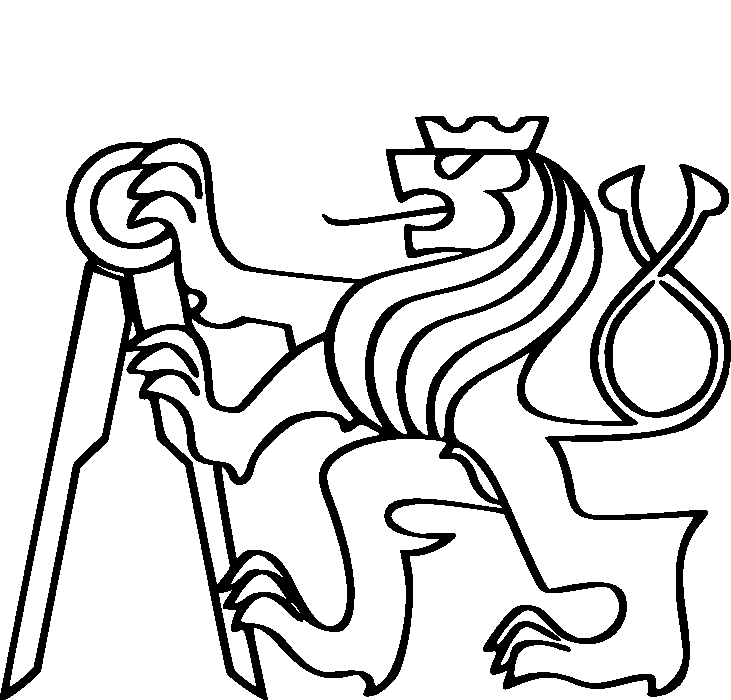
\includegraphics[scale=0.28]{../../_meta/cvut_standart.pdf}
\end{flushright}
\end{multicols}
\hrule
\vspace{0.5cm}

% ----------------------------------------------------------------------


% --- Tělo dokumentu ---------------------------------------------------
\setlength{\parindent}{0.5cm}

\section{Pracovní úkoly}

\begin{enumerate}

\item{Kryosorpční vývěva s regenerovanými zeolity + jednostupňová ROV}
\begin{enumerate}
	  \item Kryosorpční vývěvu napusťte vzduchem a nechte ustálit.
	  \item Čerpejte ROV a po hrubém ustálení tlaku začněte čerpat kryosorpční vývěvou.
	  \item Odpojte rotační olejovou vývěvu.
	  \item Čerpejte do ,,mezního`` tlaku (alespoň 1 hodinu).
	  \item Sledujte závislost tlaku na čase. 
\end{enumerate}

\item{Dvoustupňové kryosorpční čerpání}
\begin{enumerate}
	\item Kryosorpční vývěvy I a II napusťte vzduchem a nechejte ustálit. 
	\item Čerpejte první kryosorpční vývěvou (obě jsou propojené).
	\item Po hrubém ustálení tlaku začněte čerpat i druhou kryosorpční vývěvou, první odpojte.
	\item Čerpejte do ,,mezního`` tlaku (alespoň 1 hodinu).
	\item Sledujte závislost tlaku na čase.
\end{enumerate}

	\item Porovnejte dosažené výsledky pomocí obou metod a podejte kvalitativní vysvětlení.
	\item Jaký je vliv teploty v různých místech sestavy na měření tlaku?
	\item Do protokolu spočítejte příklady ze skript, str. 38--39.
\end{enumerate}

\section{Úvod}

Princip kryosorpční vývěvy je založen na vysokých sorpčních schopnostech porézních látek. Takovéto látky mají typicky velký efektivní povrch na malý objem a jednou z nich jsou zeolity, hydrogenované hlinitokřemičitany alkalických kovů a alkalických zemin. Jejich krystalická mřížka tvoří prostorovou síť mikroskopických dutinek o rozměrech v řádu jednotek nanometrů či méně. 


\section{Vypracování}
    \subsection{Teoretický úvod}				
		Jádrem kryosorpční vývěvy je tedy nádoba naplněná granulovanými zeolity. Sorpční vlastnosti zeolitů závisí hlavně na dvou parametrech - tlaku a teplotě. Za nižší teploty sorpční schopnosti zeolitů stoupají, a proto vývěvu chladíme při čerpání kapalným dusíkem. V případě, že chceme ze zeolitů dostat navázané látky, je třeba vývěvu regenerovat - typicky zahřátím na $300\unit{^\circ C}$. Při regeneraci dochází k uvolňování nahromaděných plynů, a je proto třeba, aby měla každá kryosorpční vývěva pojistný ventil. 
		
		Hlavní výhodou kryosorpčních vývěv je čistota jimi produkovaného vakua vzhledem k absenci oleje v aparatuře. Hlavní nevýhodou pak na druhou stranu je, že kryosorpční vývěvy téměř nečerpají plyny s nižší teplotou varu, než je teplota varu chladícího média. Pro kapalný dusík je teplota varu $\approx-195,8\unit{^\circ C}$ \cite{bib:tabulky}, což znamená, že se téměř nečerpá například helium, vodík či neon. Při čerpání vzduchu se tedy zvyšuje mezní tlak vzhledem k jeho složení (viz Tab.~\ref{tab:slozeni_vzduchu}).
		
% Table generated by Excel2LaTeX from sheet 'List1'
\begin{table}[htbp]
\centering
\begin{tabular}{rrrrrrrr}
\toprule
plyn  & $\mathrm{N_2}$ & $\mathrm{O_2}$ & $\mathrm{Ar}$ & $\mathrm{CO_2}$ & $\mathrm{Ne}$ & $\mathrm{He}$ & $\mathrm{Kr}$ \\
\midrule
koncentrace & 78~\% & 21~\% & 0,93~\% & 0,03~\% & 18~ppm & 5~ppm & 1~ppm \\
teplota varu $\unitb{^\circ C}$ & -195,8 & -182,9 & -185,9 &  -78,5* & -246,1 & -268,93 & -153,2 \\
\bottomrule
\end{tabular}%
\caption{Tabulka složení vzduchu, koncentrací jednotlivých složek \cite{bib:praskripta} a jejich teploty varu \cite{bib:tabulky} (* -- sublimuje, hodnoty platí za tlaku $p_R=101,3\unit{kPa}$).  }
\label{tab:slozeni_vzduchu}%
\end{table}%

		Mezi tlakem plynu nad sorbentem a množstvím plynu zachyceném v sorbentu bude v ustáleném stavu rovnováha, která závisí na teplotě. Při konstantní teplotě roste množství adsorbovaného plynu s rostoucím tlakem. Ze zachování hmotnosti plynu před a po ochlazení nám vyjde rovnost 
		\begin{equation}
			p_1 V + M Q(T_1, p_1) = p_2 V + M Q(T_2, p_2),
			\label{eq:rovnovaha}
		\end{equation}
		kde $(p_1V)$ a $(p_2V)$ jsou množství plynu v objemu $V$ na počátku a na konci čerpání, $Q(T_1, p_1)$ a $Q(T_2, p_2)$ množství plynu adsorbovaná v 1~g zeolitů na počátku (při teplotě $T_1$ a tlaku $p_1$) a na konci (při teplotě $T_2$ a tlaku $p_2$) a $M$ je hmotnost zeolitů.
	
\subsection{Postup měření}
	\subsubsection{Kryosorpční vývěva s regenerovanými zeolity + jednostupňová ROV}
		Po našem příchodu k experimentu bylo třeba zapojit rotační vývěvu tak, aby čerpala objem, a začít měřit čas. V momentu, kdy dostatečně zpomalilo klesání tlaku, jsme začali chladit kryosorpční vývěvu kapalným dusíkem, připojili ji a odpojili rotační vývěvu. Následně jsme nadále pozorovali změny tlaku a pečlivě je zapisovali.

	\subsubsection{Dvoustupňové kryosorpční čerpání}
		Rotační vývěva před naším příchodem k experimentu regenerovala zeolity v obou kryosorpčních vývěvách. V této úloze jsme uzavřeli všechny ventily vedoucí do aparatury včetně toho, kterým aparaturu čerpala rotační vývěva, a začali jsme chladit pravou kryosorpční pumpu. Ta čerpala jak vzduch ze spojovací trubice, tak vzduch uvolňující se z levé kryosorpční pumpy v důsledku poklesu tlaku. V momentu, kdy se tlak ustálil okolo 5~Pa, jsme uzavřeli ventil vedoucí k pravé kryosorpční pumpě a chladicí nádobu s kapalným dusíkem jsme přendali na levou. Dále jsme sledovali průběh tlaku v aparatuře Piraniho manometrem a tlaky v závislosti na čase zapisovali.
	
\subsection{Naměřené hodnoty}
	Naměřené hodnoty z obou dvou měření jsou vyneseny do grafu na Obr.~\ref{fig:g_tlak}. Při rotačně-kryosorpčním čerpání vidíme okolo 9. minuty jasný pokles tlaku, který byl způsoben připojením a chlazením kryosorpční vývěvy. U kryosorpčně-kryosorpčního čerpání je patrné odpojení pravé vývěvy okolo 45. minuty.
	
	\begin{figure}[h!]
		\begin{center}
			%\vspace*{-0.5cm}
			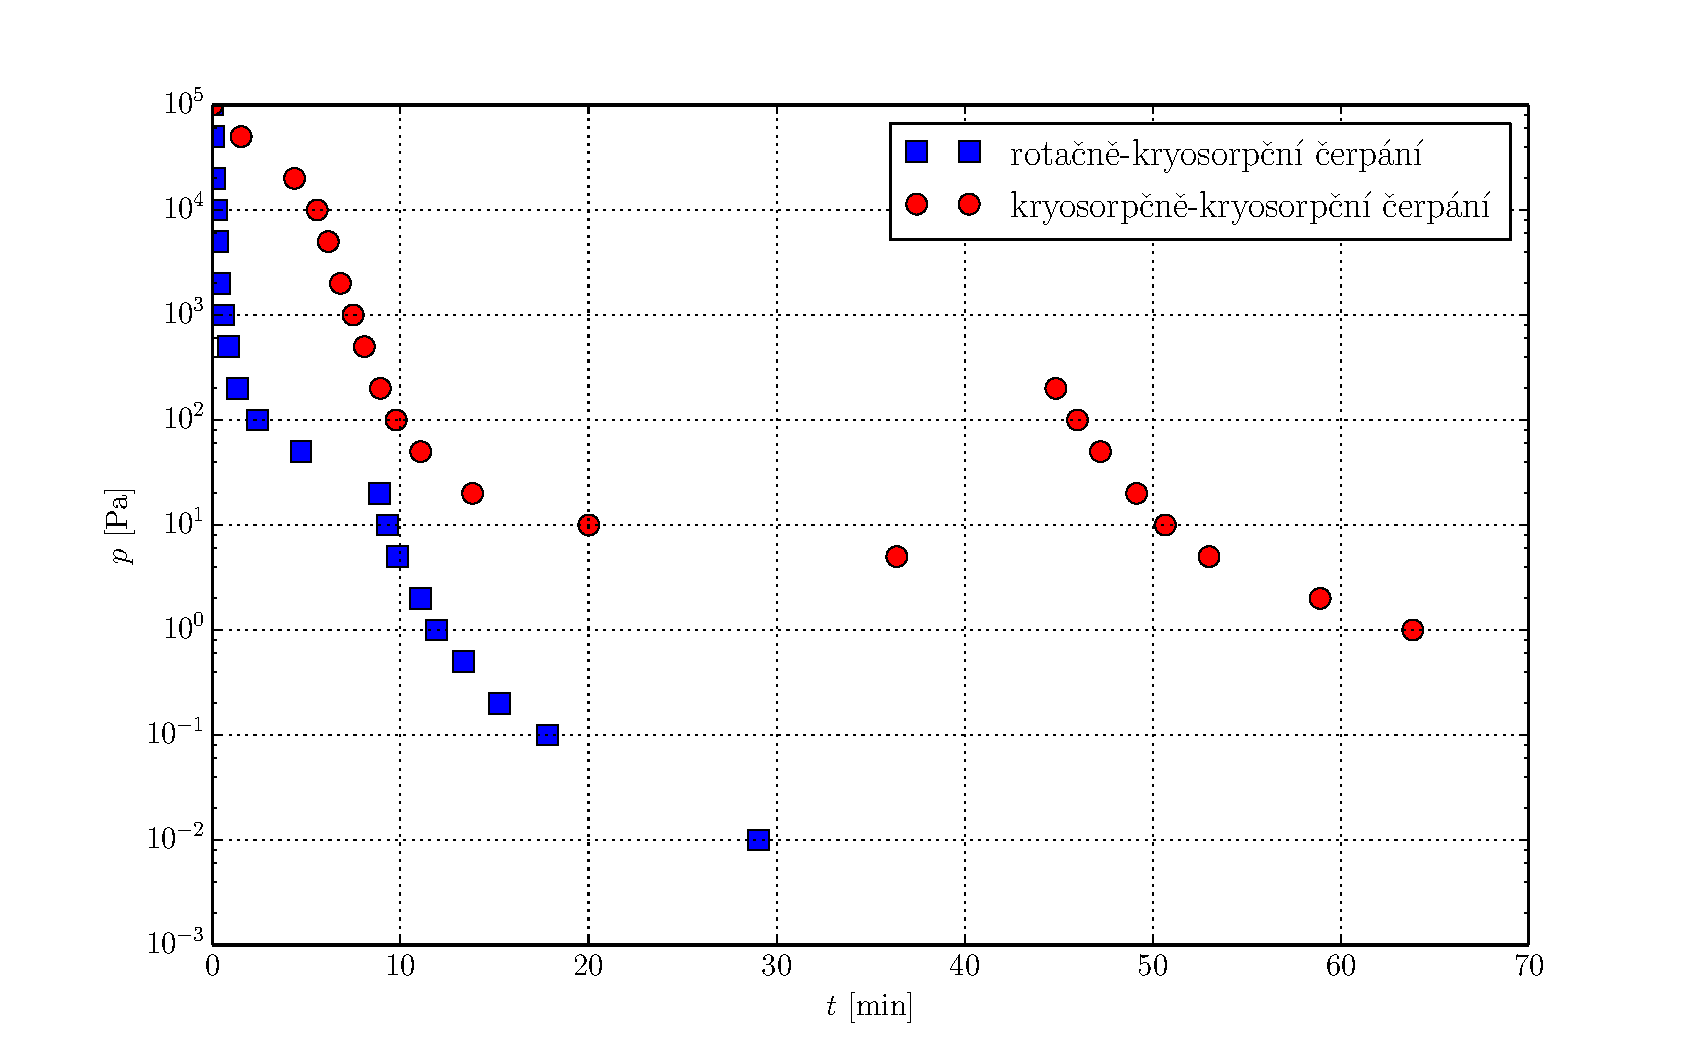
\includegraphics[width=\linewidth]{../plt/01_kryorot.pdf}
			\vspace*{-0,7cm}
			\caption{Naměřené hodnoty závislosti tlaku v recipientu $p$ na čase $t$ při rotačně-kryosorpčním a kryosorpčně-kryosorpčním čerpání. }
			\label{fig:g_tlak}
		\end{center}
	\end{figure}
			
\subsection{Diskuse}
	\subsubsection{Kryosorpční vývěva s regenerovanými zeolity + jednostupňová ROV}
		Z grafu na Obr.~\ref{fig:g_tlak} je patrné, v jaký moment došlo k přepnutí mezi ROV a kryosorpční vývěvou. Okamžitě po přepnutí jsme nepozorovali dočasné stoupnutí tlaku jako v druhé úloze. Tuto skutečnost připisujeme faktu, že jsme začali kryosorpční vývěvu chladit o chvilku dříve, než jsme odpojili vývěvu rotační, což vedlo k jejímu hladkému nástupu a nebylo třeba čekat na její zchlazení.
		
		Při čerpání rotační olejovou vývěvou se dalo čekat o trochu déle, ale neočekáváme, že by tlak klesl o moc níže. Poslední naměřené hodnota tlaku není tlakem mezním, což tentokrát není způsobeno nedostatečně dlouhým časem čerpání, nýbrž příliš malým rozsahem použitého vakuometru, který nižší hodnoty tlaku neukazoval. Prostudujeme-li pečlivěji graf a provedeme-li myšlenkovou extrapolaci křivky dále v čase, jeví se rozumné předpokládat, že bychom se dostali ještě například o řád níže než na minimální zaznamenanou hodnotu $10^{-2}\unit{Pa}$.
		
	\subsubsection{Dvoustupňové kryosorpční čerpání}
		V této části pokusu jsme hned na začátku udělali zásadní chybu. Ač byly obě kryosorpční vývěvy zregenerované čerpáním objemu pomocí ROV, nebylo to nic platné, jelikož jsme čerpání pravou kryosorpční vývěvou zahájili s otevřeným ventilem, kterým byla původně připojena ROV, ale který už vedl na vzduch. Velice rychle jsme tím pádem nasytili zeolity v druhé z vývěv. Prodloužili jsme si tím měření o více než hodinu, jelikož bylo potřeba znovu zahřát a zregenerovat pravou vývěvu.
		
		Nejprve jsme tedy nechali vývěvu ve vodě o pokojové teplotě, aby se trochu ohřála. Poté jsme z ní nádobu s vodou sundali a nožem jsme odlámali led, který se na vývěvě za dobu ohřívání vytvořil. Následně jsme na vývěvu nasadili ohřívač, který ji ještě trochu ohřál a nakonec jsme ještě znovu vyčerpali objem ROV. Po asi hodině času jsme vývěvu prohlásili za dostatečně zregenerovanou, ale je třeba dbát toho, že naše závěry nemusí být na základě této události zcela korektní. Nemůžeme totiž dost dobře odlišit, nakolik za případné rozdíly oproti prvnímu měření může kryosorpčně-kryosorpční čerpání a nakolik jsme tento rozdíl způsobili my naší neopatrností.
		
		Zajímavostí je, že kryosorpčně-kryosorpční čerpání by nemělo být schopno dosahovat tak nízkých tlaků, jako se nám s ním podařilo naměřit. My jsme i přes výše zmíněnou chybu byli schopni dosáhnout při pokusu tlaku mírně pod 1~Pa. Jedním z faktorů, který by mohl hrát roli, může být to, že Piraniho tepelný vakuometr byl cejchován na vzduch, zatímco v naší aparatuře je přítomno převážně helium a jiné plyny, které kryosorpční vývěvy nečerpají. Druhou možností je, že bylo měření tlaku Piraniho vakuometrem ovlivněno teplotním gradientem, který vznikl v aparatuře mezi kryogenní vývěvou a místem, kde byl tlak měřený. Vzhledem k tomu, že naměřený údaj tlaku závisí také na $\sqrt{T}$, mohla se teplota přímo projevit na naměřeném tlaku. 
	
		Dalším pozorovaným jevem při tomto měření byl tlakový nárůst bezprostředně po odpojení pravé kryosorpční vývěvy. Usuzujeme, že se tak stalo vzhledem k tomu, že levá vývěva uvolňovala daným teplotně-tlakovým podmínkám odpovídající množství plynu, které ale nemělo kam odcházet, jelikož pravá vývěva už byla odpojena. Tlak následně začal klesat, když jsme začali chladit levou vývěvu, jelikož byly plyny opět adsorbovány zpět do ní. Stoupnutí tlaku tedy přímo odpovídá době, jakou nám trvalo zchladit zeolity v levé vývěvě.
	
	\subsubsection{Porovnání obou sestavení}
		Z grafu na Obr.~\ref{fig:g_tlak} je jasně patrné, že při rotačně-kryosorpčním čerpání jsme dosáhli dramaticky nižšího tlaku nežli při čerpání kryosorpčně-kryosorpčním. Jak již bylo v diskusi zmíněno, je to možná zaviněno naším pochybením a veškeré závěry tedy můžou být chybné. Předpokládejme ale, že tomu tak není. Potom je rozumné usuzovat, že bylo rotačně-kryosorpčním čerpáním dosaženo lepších výsledků vzhledem k tomu, že přečerpání ROV odčerpalo přibližně rovnoměrně všechny složky atmosferického vzduchu na podobné úrovně. Kryosorpční vývěva, která poté začala čerpat, tím pádem byla schopna odčerpat všechny plyny ještě více, až na relativně malé množství některých plynů (helium, neon, ...). 
		
		V případě předčerpávání druhou kryosorpční vývěvou se však tyto plyny z čerpaného objemu neodčerpaly téměř vůbec. Po odpojení pravé vývěvy a zahájení chlazení té levé znovu nedošlo k odčerpání těchto plynů, a proto zůstal tlak na vyšší úrovni než v předchozím sestavení.
		
		Z příkladů spočítaných v příloze vychází, že bychom pomocí kryosorpčně-kryosorpčního čerpání měli být schopni dosahovat tlaků okolo $10^{-6}\unit{Pa}$. Je však třeba si uvědomit, že v příkladu počítáme s čerpáním dusíku, který kryosorpční vývěvy čerpají dokonale, a ne vzduchu.
						
\section{Závěr}
	Čerpali jsme pomocí kryosorpční vývěvy regenerované zeolity a jednostupňovou rotační olejovou vývěvou.
	
	Předčerpání ROV jsme nahradili další kryosorpční vývěvou a po menších problémech jsme si vyzkoušeli dvoustupňové kryosorpční čerpání.
	
	Porovnali jsme výsledky dosažené pomocí obou metod a podali jsme kvalitativní vysvětlení.
	
	Diskutovali jsme vliv teploty v různých místech sestavy na měření tlaku.
	
	Do protokolu jsme spočítali příklady ze skript, viz přílohy.

	
\section {Použitá literatura}
% --- Literatura a reference -------------------------------------------
\begingroup
\renewcommand{\section}[2]{}

\begin{thebibliography}{9}

\bibitem{bib:chyby} Kolektiv KF, \emph{Chyby měření} [Online], [cit. \today] \newline http://praktikum.fjfi.cvut.cz/documents/chybynav/chyby-o.pdf

\bibitem{bib:praskripta}Král, J.: \emph{Cvičení z vakuové techniky},
Vydavatelství ČVUT, Praha, 1996

%\bibitem{bib:tlak}ČHMÚ: \emph{Aktuální informace o počasí na území České republiky}, {[}online{]}, {[}cit. \today{]},\\ http://pr-asv.chmi.cz/synopy-map/pocasisp.php?ukazatel=stanice\&pozadi=\&pozadi=mapareg\&graf=ano

\bibitem{bib:tabulky} J. Mikulčák a kol., Matematické, fyzikální a chemické tabulky \& vzorce. Prometheus,
Praha 2009.\newline
ISBN 978-80-7196-264-9

\end{thebibliography}
\endgroup
% ----------------------------------------------------------------------
\setcounter{equation}{0}
\numberwithin{equation}{section}

\clearpage
\part*{Přílohy}

%%%%\section{Domácí příprava}
%%%%	Domácí příprava je přiložena k protokolu.
%%%%\clearpage
%%%\section{Statistické zpracování dat}
%%%	Pro statistické zpracování využíváme aritmetického průměru:
%%%	\begin{equation} \label{eq:aritmeticky_prumer}
%%%	\overline{x} = \frac{1}{n}\sum\limits_{i=1}^{n}x_i,
%%%	\end{equation}
%%%
%%%%	jehož směrodatnou odchylku spočítáme jako 
%%%%	\begin{equation} \label{eq:smodch_aritmetickeho_prumeru}
%%%%	\sigma_0 = \sqrt{\frac{1}{n} \sum\limits_{i=1}^{n}\left( x_i - \overline{x} \right)^2 },
%%%%	\end{equation}
%%%%	
%%%%	kde $ x_i $ jsou jednotlivé naměřené hodnoty, $ n $ je počet měření, $ \overline{x} $ aritmetický průměr a $ \sigma_0 $ jeho chyba \cite{bib:chyby}.
%%%	
%%%	
%%%	jehož chybu spočítáme jako 
%%%	\begin{equation} \label{eq:chyba_aritmetickeho_prumeru}
%%%	\sigma_0 = \sqrt{\frac{1}{n(n-1)} \sum\limits_{i=1}^{n}\left( x_i - \overline{x} \right)^2 },
%%%	\end{equation}
%%%	
%%%	kde $ x_i $ jsou jednotlivé naměřené hodnoty, $ n $ je počet měření, $ \overline{x} $ aritmetický průměr a $ \sigma_0 $ jeho chyba \cite{bib:chyby}.
%%%%	
%%%Při nepřímém měření počítáme hodnotu s chybou dle následujících vztahů:
%%%	\begin{equation}
%%%	u = f(x, y, z, \ldots),
%%%	\end{equation}
%%%	\begin{displaymath}
%%%	x = (\overline{x} \pm \sigma_x), \qquad
%%%	y = (\overline{y} \pm \sigma_y), \qquad
%%%	z = (\overline{z} \pm \sigma_z), \qquad
%%%	\ldots,
%%%	\end{displaymath}
%%%	
%%%	kde $ u $ je veličina, kterou určujeme nepřímo z měřených veličin $ x, y, z, \ldots $ 
%%%	
%%%	Pak
%%%	\begin{displaymath}
%%%	\overline{u} = f(\overline{x}, \overline{y}, \overline{z}, \ldots),
%%%	\end{displaymath}
%%%	\begin{equation}\label{eq:chyba_neprime_mereni}
%%%	\sigma_u = \sqrt{\left( \frac{\partial f}{\partial x} \right)^2 \sigma^2_x + \left( \frac{\partial f}{\partial y} \right)^2 \sigma^2_y + \left( \frac{\partial f}{\partial z} \right)^2 \sigma^2_z + \ldots},
%%%	\end{equation}
%%%	\begin{displaymath}
%%%	u = (\overline{u} \pm \sigma_ u).
%%%	\end{displaymath}
%%	
%V případě, že máme několik různě přesných měření stejné veličiny, používáme vztah pro vážený průměr:
%	\begin{equation} 
%	\overline{x}=\frac{\sum\limits_{i=1}^{n}p_{i}x_{i}}{\sum\limits_{i=1}^{n}p_{i}},
%	\end{equation}
%	
%	kde $\overline{x}$ je vážený průměr, $x_{i}$ jsou jednotlivá měření a pro $p_{i}$ platí
%	 
%	\begin{equation}
%	p_{i}=\frac{1}{\sigma_{i}^{2}},
%	\end{equation}
%	
%	kde $\sigma_{i}$ jsou jednotlivé chyby daných měření.
%	 
%	Celkovou chybu tedy vypočítáme ze vztahu
%	\begin{equation} \label{eq:vazeny_prumer}
%	\sigma_{0}=\sqrt{\frac{1}{\sum\limits_{i=1}^{n}p_{i}}}.
%	\end{equation}
%
%\subsubsection{Metoda nejmenších čtverců}
%Snažíme-li se metodou nejmenších čtverců proložit data lineární závislostí $Y_i = ax_i+b$, dosazujeme hodnoty $x_i, y_i$ a snažíme se najít parametry $a$ a $b$ tak, aby byl součet všech kvadratických odchylek $\Delta Y_i^2$ minimální. Toho dosáhneme pomocí následujících vzorců \cite{bib:ctverce} :
%\begin{equation}\label{eq:ctverce_a}
%		a = \frac{n\sum\limits_{i=1}^{n}{x_i y_i}  - \sum\limits_{i=1}^{n}{x_i}\sum\limits_{i=1}^{n}{y_i}}{n\sum\limits_{i=1}^{n}{x_i^2}  - \left(\sum\limits_{i=1}^{n}{x_i}\right)^2}, \qquad \qquad
%		\sigma_a = \sqrt{\frac{n\sum\limits_{i=1}^{n}{(y_i - Y_i)^2} }{(n-2)\left(\sum\limits_{i=1}^{n}{x_i^2}  - \left(\sum\limits_{i=1}^{n}{x_i}\right)^2\right)}},
%\end{equation}
%
%\begin{equation}\label{eq:ctverce_b}
%		b = \frac{\sum\limits_{i=1}^{n}{x_i^2} \sum\limits_{i=1}^{n}{y_i}  - \sum\limits_{i=1}^{n}{x_i}\sum\limits_{i=1}^{n}{x_i y_i}}{n\sum\limits_{i=1}^{n}{x_i^2}  - \left(\sum\limits_{i=1}^{n}{x_i}\right)^2}, \qquad \qquad
%		\sigma_b = \sqrt{\frac{\sum\limits_{i=1}^{n}{x_i^2}\sum\limits_{i=1}^{n}{(y_i - Y_i)^2} }{n(n-2)\left(\sum\limits_{i=1}^{n}{x_i^2}  - \left(\sum\limits_{i=1}^{n}{x_i}\right)^2\right)}}.
%\end{equation}
%\clearpage
\subsection{Příklady}
\subsubsection{Příklad 1}
\textbf{Zadání:} \emph{Recipient o objemu $20$ litrů je čerpán jednou kryosorpční vývěvou. Ve vývěvě je $500\unit{g}$ zeolitu typu $\unit{5A}$. Aparatura s regenerovanými zeolity v kryosorpční vývěvě je na počátku naplněna dusíkem a ponechána, aby se v ní ustálily poměry při atmosférickém tlaku a teplotě $20\unit{^\circ C}$. Potom jsou zeolity ochlazeny na $-195\unit{^\circ C}$. Za předpokladu těsné aparatury a při zanedbání desorpce ze stěn recipientu určete dosažitelný mezní tlak.}

\vspace{0.5cm}
Z grafu na Obr.~\ref{fig:s_1} je možné odečíst hodnotu 
\begin{equation}
	Q(20\unit{^\circ C}, 10^{5}\unit{Pa}) = 10^{3}\unit{Pa\cdot l\cdot g^{-1}}.
\end{equation} 
Dosadíme-li tyto hodnoty do vztahu (\ref{eq:rovnovaha}), dostaneme rovnici (v jednotkách $\unit{Pa\cdot l}$)
\begin{equation}
10^{5}\cdot 20 + 500\cdot 1000 = p_2\cdot 20 + 500\cdot Q(-195\unit{^\circ C}, p_2).
\label{eq:pr1}
\end{equation}
Zanedbáme-li vzhledem k předpokladu malé velikosti $p_2$ první člen na pravé straně, dostaneme
\begin{equation}
	Q(-195\unit{^\circ C}, p_2) = 5\cdot 10^3\unit{Pa\cdot l\cdot g^{-1}},
\end{equation}
z čehož plyne hledaný výsledek jako 
\begin{equation}
	 p_2 = 0,5\unit{Pa}.
\end{equation}


\begin{figure}[h!]
\centering
\begin{minipage}[t]{.43\textwidth}
\centering
				
				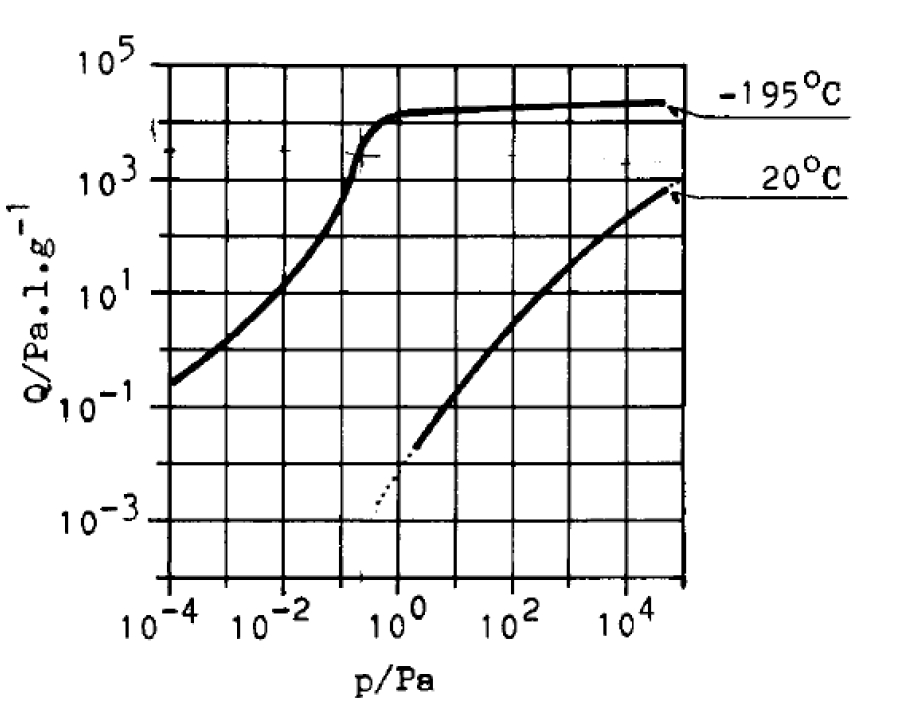
\includegraphics[scale=0.35]{../att/tlak_origo}
				\caption{Závislost množství dusíku adsorbovaného na zeolitu typu 5A na tlaku $p$ nad zeolitem pro $20\unit{^\circ C}$ a $-195\unit{^\circ C}$ - převzato z \cite{bib:praskripta}.}
				\label{fig:s_1}
\end{minipage}%
\hfill
\begin{minipage}[t]{.45\textwidth}
\centering
				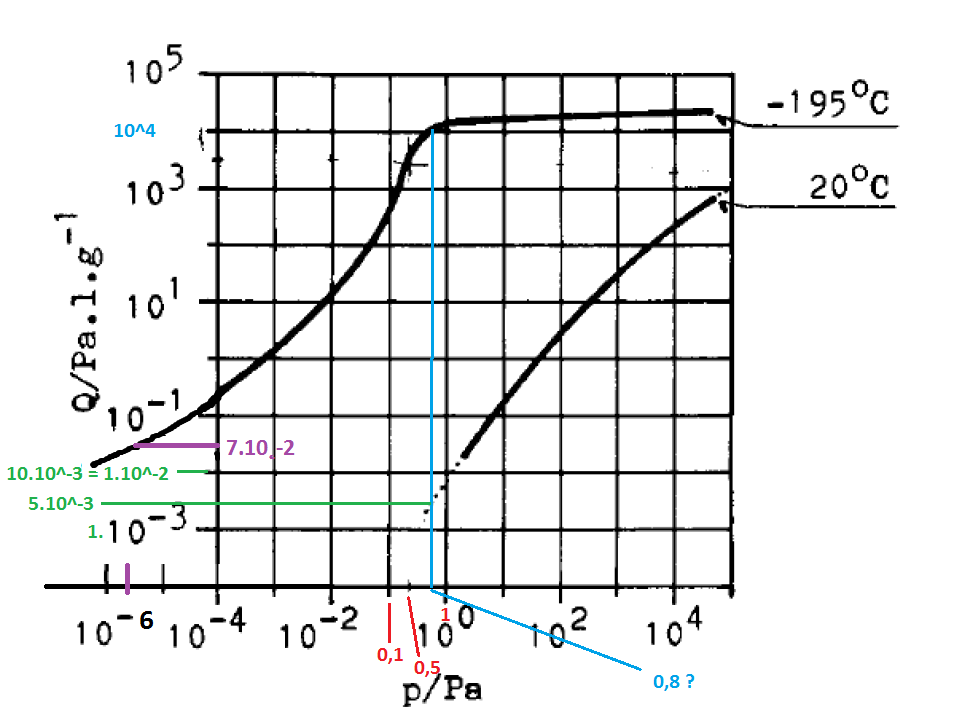
\includegraphics[scale=0.35]{../att/tlak_muj}
				\caption{Schématický nákres vedlejšího grafu pro myšlenkovou extrapolaci hodnot (vlastní tvorba).}
				\label{fig:s_2}
\end{minipage}
\end{figure}

\clearpage
\subsubsection{Příklad 2}
\textbf{Zadání:} \emph{Recipient o objemu $20$ litrů je čerpán dvoustupňově kryosorpčními vývěvami. Každá ze dvou vývěv obsahuje $250\unit{g}$ zeolitu typu $\unit{5A}$. Aparatura s regenerovanými zeolity ve vývěvách je na počátku naplněna dusíkem a ponechána, aby se v ní ustálily poměry při atmosférickém tlaku a $20\unit{^\circ C}$. Potom jsou zeolity v první vývěvě ochlazeny na  $ -195\unit{^\circ C}$, přičemž druhá, nechlazená vývěva je spojena s recipientem. Po delší době, až se nastaví nová rovnováha mezi dusíkem adsorbovaným v teplých zeolitech, dusíkem adsorbovaným ve studených zeolitech a plynným dusíkem v aparatuře, oddělí se první vývěva se studenými
zeolity od recipientu. Objem aparatury se bude dále čerpat zeolity ve druhé vývěvě, která se ochladí na  $ -195\unit{^\circ C}$. Za předpokladu těsné aparatury a při zanedbání desorpce ze stěn a zanedbání objemu odstavené první vývěvy určete tlak dusíku v aparatuře po prvním stupni čerpání a oceňte konečný mezní tlak v recipientu.}

\vspace{0.5cm}
Opět budeme vycházet ze vztahu (\ref{eq:rovnovaha}). Pokud analogicky předchozí úloze dosadíme pro první ochlazení, dostaneme
\begin{equation}
p_A\cdot V + 2\cdot M\cdot Q(20\unit{^\circ C}, p_A) = p_2\cdot V + M\cdot  Q(20\unit{^\circ C}, p_2) + M\cdot  Q(-195\unit{^\circ C}, p_2)
\label{eq:pr2a}
\end{equation}
a vzhledem k odhadu dostatečně nízkého tlaku můžeme opět zanedbat první a druhý člen na pravé straně. Z Obr.~\ref{fig:s_1} můžeme (stejně jako v prvním příkladě) odečíst hodnotu
\begin{equation}
	Q(20\unit{^\circ C}, 10^{5}\unit{Pa}) = 10^{3}\unit{Pa\cdot l\cdot g^{-1}},
\end{equation}
což nás přivede k rovnici
\begin{equation}
	10^5\cdot 20 + 2\cdot 250\cdot 10^3 = 250\cdot Q(-195\unit{^\circ C}, p_2),
\end{equation}
z čehož jde vyjádřit za pomoci Obr.~\ref{fig:s_1}
\begin{equation}
	Q(-195\unit{^\circ C}, p_2) = 10^4\unit{Pa\cdot l\cdot g^{-1}} \implies p_2 = 0,8\unit{Pa},
\end{equation}
což nás podle stejného grafu zavede ke zjištění, že
\begin{equation}
	 Q(20\unit{^\circ C}, p_2) = 6\cdot 10^{-3}\unit{Pa\cdot l\cdot g^{-1}}.
\end{equation}
Následným dosazením do rovnice (\ref{eq:rovnovaha}) pro druhé zchlazení dostáváme
\begin{equation}
	p_2\cdot V+M\cdot Q(20\unit{^\circ C}, p_2) = p_3\cdot V+M\cdot Q(-195\unit{^\circ C}, p_3),
\end{equation}
což v číslech odpovídá (při zanedbání prvního členu na pravé straně) rovnici
\begin{equation}
	0,8\cdot 20+250\cdot 6\cdot 10^{-3} = 250\cdot Q(-195\unit{^\circ C}, p_3),
\end{equation}
ze které vyplývá
\begin{equation}
	Q(-195\unit{^\circ C}, p_3) = 7\cdot 10^{-2} \unit{Pa\cdot l\cdot g^{-1}}.
\end{equation}
Pro takovouto hodnotu již na grafu tlak neodečteme, ale můžeme při myšlenkové extrapolaci dospět k hodnotě $p_3\approx 10^{-6}\unit{Pa}$, jak je ilustrováno na schématickém nákresu na Obr.~\ref{fig:s_2}. Ze stejného obrázku je ale vidět, že bychom při vhodném do\emph{malování} křivky mohli dospět k (i řádově) jiným hodnotám. Tento výsledek proto bereme pouze jako orientační.
	
\clearpage
\subsection{Tabulky a grafy}

\begin{table}[h!]
\begin{minipage} [c]{.45\linewidth}
\centering
\vspace{1.05cm}
\begin{tabular}{|r|r|}
\hline
  \boldmath{}\textbf{$p\unitb{Pa}$}\unboldmath{}\ & \boldmath{}\textbf{$t\unitb{s}$}\unboldmath{} \\
       \hline
       1,00E+05 & 0,00 \\\hline
       5,00E+04 & 4,23 \\\hline
       2,00E+04 & 8,11 \\\hline
       1,00E+04 & 12,67 \\\hline
       5,00E+03 & 17,77 \\\hline
       2,00E+03 & 23,88 \\\hline
       1,00E+03 & 35,18 \\\hline
       5,00E+02 & 50,98 \\\hline
       2,00E+02 & 81,34 \\\hline
       1,00E+02 & 145,11 \\\hline
       5,00E+01 & 282,90 \\\hline
       2,00E+01 & 534,00 \\\hline
       1,00E+01 & 560,00 \\\hline
       5,00E+00 & 590,00 \\\hline
       2,00E+00 & 664,00 \\\hline
       1,00E+00 & 714,02 \\\hline
       5,00E-01 & 800,73 \\\hline
       2,00E-01 & 915,37 \\\hline
       1,00E-01 & 1068,97 \\\hline
       1,00E-02 & 1742,38 \\\hline
      
   \end{tabular}
     \caption{Naměřené hodnoty za rotačně-kryosorpčního čerpání; $p$ je tlak naměřený Piraniho vakuometrem, $t$ čas.} 
     \label{tab:kryorot}
\end{minipage}
\hspace{0.5cm} 
\begin{minipage}[c]{.45\linewidth}
\centering
\begin{tabular}{|r|r|}
\hline
\boldmath{}\textbf{$p\unitb{Pa}$}\unboldmath{}\ & \boldmath{}\textbf{$t\unitb{s}$}\unboldmath{}\\
     \hline
    1,00E+05 & 0,00 \\ \hline
    5,00E+04 & 91,70 \\ \hline
    2,00E+04 & 262,23 \\ \hline
    1,00E+04 & 334,43 \\ \hline
    5,00E+03 & 369,83 \\ \hline
    2,00E+03 & 408,61 \\ \hline
    1,00E+03 & 449,19 \\ \hline
    5,00E+02 & 484,79 \\ \hline
    2,00E+02 & 535,96 \\ \hline
    1,00E+02 & 586,23 \\ \hline
    5,00E+01 & 664,72 \\ \hline
    2,00E+01 & 830,11 \\ \hline
    1,00E+01 & 1200,95 \\ \hline
    5,00E+00 & 2183,57 \\ \hline
    2,00E+02 & 2691,11 \\ \hline
    1,00E+02 & 2759,82 \\ \hline
    5,00E+01 & 2833,24 \\ \hline
    2,00E+01 & 2948,68 \\ \hline
    1,00E+01 & 3040,30 \\ \hline
    5,00E+00 & 3179,69 \\ \hline
    2,00E+00 & 3534,09 \\ \hline
    1,00E+00 & 3829,66 \\ \hline
    
      \end{tabular}
    \caption{Naměřené hodnoty za kryosorpčně-kryosorpčního čerpání; $p$ je tlak naměřený Piraniho vakuometrem, $t$ čas.}
    \label{tab:kryo+kryo}    
\end{minipage}
\end{table}

%\clearpage
%\subsection{Schémata}
%	
%	\begin{figure}[h!]
%	\centering
%			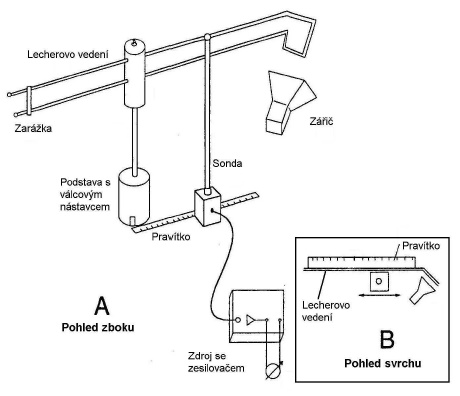
\includegraphics[width=13cm]{att/lecherovo_vedeni.jpg}
%			\caption{Experiment s Lecherovým vedením (převzato z  \cite{bib:zadani}). }
%			\label{fig:lecherovo_vlneni}
%	\end{figure}	
%	
%\clearpage
% --- Konec dokumentu --------------------------------------------------

\end{document}

